\documentclass{llncs}
%\documentclass{journallet}
\usepackage{graphicx,amssymb,amsmath,amsfonts,fancyhdr,wrapfig,here}
\usepackage{times}
\usepackage{subfigure}
\usepackage{latexsym}
\usepackage{bbm}
\usepackage{enumerate}
\usepackage{caption}
\usepackage{lineno}

%-------------- Macros and Definitions -----------------------------------

\newtheorem{observation}{Observation}

\newcommand{\NN}{\mathbb{N}} %  set of natural numbers
\newcommand{\ZZ}{\mathbb{Z}} %  set of integer number
\newcommand{\RR}{\mathbb{R}} %  set of real numbers
\newcommand{\SH}{\mathbb{S}} %  set of unit vectors
\newcommand{\HH}{{\cal H}} %  Calligraphic H
\newcommand{\PP}{{\cal P}} %  Calligraphic P
\newcommand{\DD}{{\cal D}} %  Calligraphic Q


\def\etal{{et~al.}}
\def\ie{{i.e.}}
\def\eg{{e.g.}}
\def\slope{{\rm slope}}

\def \proof {\par \noindent {\bf Proof.}\hskip 5pt}
\def \endproof {\hfill $\Box$ \smallskip}

\pagestyle{fancy}
\fancyhead[RO,LE]{\thepage}
\fancyhead[LO]{\it\nouppercase Realization of simply connected polygonal linkages}
\fancyhead[RE]{\it\nouppercase\leftmark}
\renewcommand{\headrulewidth}{0pt} \fancyfoot{}


%---------------------- Title ---------------------------------------------

\title{Realizations of simply connected polygonal linkages}

%\author{Clinton Bowen\thanks{Department of Mathematics, California State University, Northridge, CA, %USA. \texttt{clinton.bowen@my.csun.edu} and \texttt{csaba.toth@csun.edu}}
%\and Csaba~D.~T\'oth$^*$}


\author{Clinton Bowen\inst{1} \and Csaba~D.~T\'oth\inst{1}}
\institute{Department of Mathematics, California State University, Northridge, CA, USA.\\
\email{clinton.bowen@my.csun.edu csaba.toth@csun.edu}}



\begin{document}
\linenumbers
\maketitle

\begin{abstract}
We consider two variants of the fundamental question whether a simply connected flexible combinatorial structure can be realized in Euclidean space, motivated by applications in molecular biology and self-assembly. Two models are considered: body-and-joint frameworks and contact graphs of disks in the plane. We show that it is NP-hard to decide (1) whether a given polygonal linkage (body-and-bar framework) is realizable in the plane when the bodies are convex polygons and their contact graph is a tree; (2) whether a given tree is the contact graph of circular disks of given radii in the plane.
\end{abstract}



\section{Introduction}\label{sec:intro}

Complex structures in nature are often composed of elementary pieces that obey simple local composition rules. Molecular biology, nanomanufacturing, and self-assembly are prime examples. Mathematical models for this phenomenon typically rely on rigidity theory and formal languages. In this paper, we study the realizability of complex structures that are given with a local specification. We consider two models in Euclidean plane.

\begin{enumerate}
\item A {\bf polygonal linkage} is a set $\PP$ of convex polygons, and a set $H$ of hinges,
where each hinge $h\in H$ corresponds to two points on the boundary of two distinct polygons.
A \emph{realization} of a polygonal linkage is an interior-disjoint placement of congruent copies of the polygons in $\PP$ such that the points corresponding to each hinge are identified (Fig.~\ref{fig:1}, left).
\item A {\bf disk arrangement} is a set $\DD$ of pairwise interior-disjoint disks in the plane. The contact graph of a disk arrangement $\DD$ is a graph $G=(\DD,E)$ where two vertices are adjacent if the corresponding disks intersect (kiss). A \emph{realization} of a vertex-weighted graph $G$ as a contact graph of disks is a disk arrangement whose contact graph is $G$ and the radius of each disk is the corresponding vertex weight.
\end{enumerate}

\begin{figure}[htbp]
  \centering
 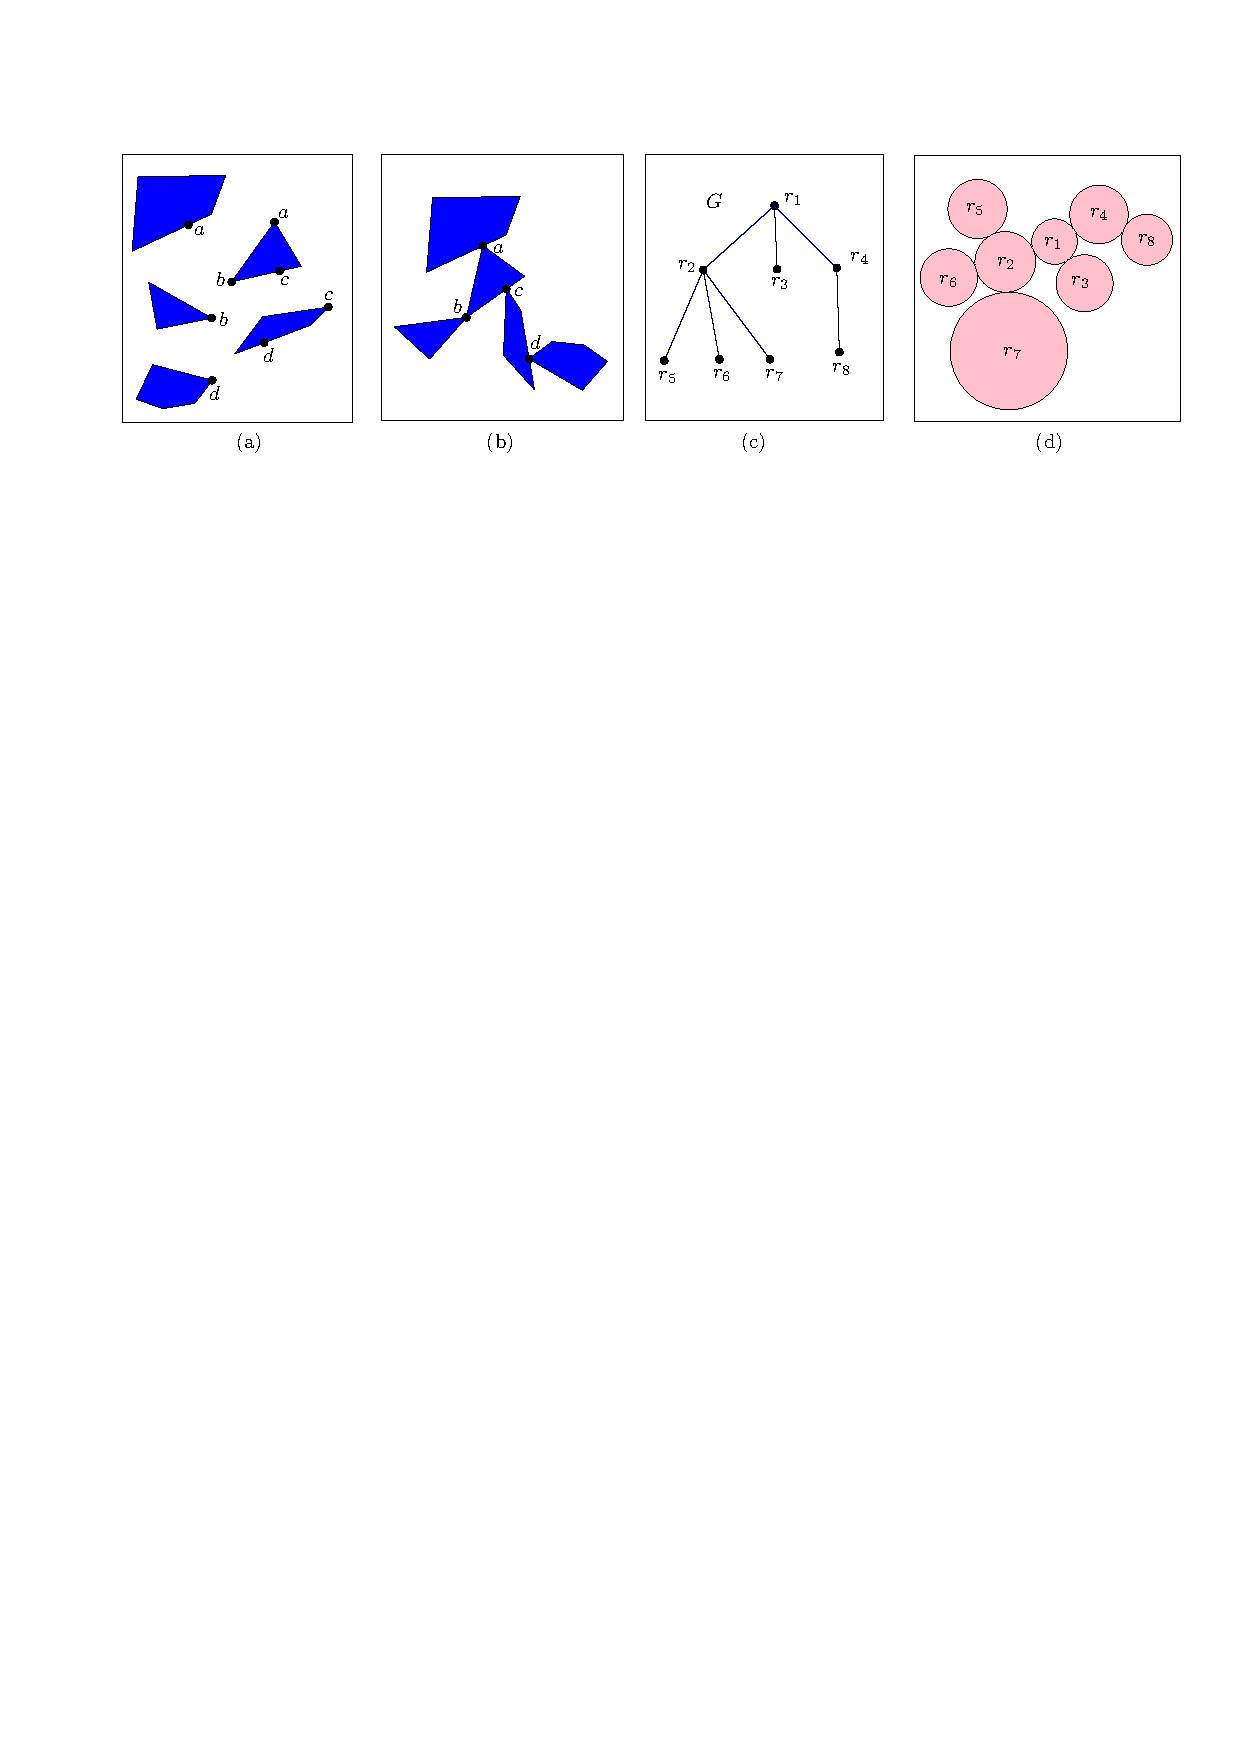
\includegraphics[width=0.95\textwidth]{fig1}
\caption{\small (a) A set of convex polygons and hinges. (b) A realization of the polygonal linkage from (a).
(c) A graph $G$ with vertex weights $r_1,\ldots , r_8$. (d) A disk arrangement that realizes the weighted graph $G$
 as a contact graph with radii equal to the corresponding weights.}
  \label{fig:1}
\end{figure}

Each model has two variants, depending on whether \emph{reflection} is allowed for the realization of each piece independently. For polygonal linkages, an \emph{oriented realization} requires translated and rotated copies of the polygons in $\PP$ (i.e., reflection is not allowed). An \emph{ordered contact graph} for a disk arrangement is a \emph{plane graph} $G$, where the circular order of the neighbors of each vertex is specified, and an \emph{oriented realization} is disk arrangement with the given ordered contact graph.

The \emph{realizability} problem for a polygonal linkage asks whether a given polygonal linkage has a realization (resp., orientated realization). For a weighted planar (resp., plane) graph,, it asks whether the graph is
the contact graph (resp., ordered contact graph) of some disk arrangement with specified radii. These problems, in general, are known to be NP-hard. Specifically, it is NP-hard to decide whether a given planar (or plane) graph can be embedded in $\RR^2$ with given edge lengths~\cite{CDD+10,EW90}. Since an edge of given length can be modeled by a suitably long and skinny rhombus, the realizability of polygonal linkages is also NP-hard. The recognition of the contact graphs of unit disks in the plane (a.k.a. coin graphs) is NP-hard~\cite{BK98}, and so the realizability of weighted graphs as contact graphs of disks is also NP-hard. However, previous reductions crucially rely on configurations with high genus: the planar graphs in~\cite{CDD+10,EW90} and the coin graphs in~\cite{BK98} have many cycles.

In this paper, we consider the above four realizability problems when the union of the polygons (resp., disks) in the desired configuration is simply connected (i.e., contractible). That is, the contact graph of the disks is a tree, or the ``hinge graph'' of the polygonal linkage is a tree (the vertices in the \emph{hinge graph} are the polygons in $\PP$, and edges represent a hinge between two polygons). Our main result is that realizability remains NP-hard when restricted to simply connected structures.

\begin{theorem}\label{thm:hinge}
It is NP-complete to decide whether a polygonal linkage whose hinge graph is a tree can be realized (both with and without orientation).
\end{theorem}

\begin{theorem}\label{thm:disk}
It is NP-complete to decide whether a given tree (resp., plane tree) with positive vertex weights
is the contact graph (resp., ordered contact graph) of a disk arrangements with specified radii.
\end{theorem}

The unoriented versions, where the underlying graph (hinge graph or contact graph) is a tree can easily be handled with the logic engine method (Section~\ref{sec:logic}). We prove Theorem~\ref{thm:hinge} for \emph{oriented} realizations with a reduction from {\sc Planar-3SAT} (Section~\ref{sec:hinge}), and then reduce the realizability of ordered contact trees to the oriented realization of polygonal linkages by simulating polygons with arrangements of disks (Section~\ref{sec:disk}).

\smallskip\noindent{\bf Related Previous Work.}
Polygonal linkages (or body-and-joint frameworks) are a generalization of classical linkages (bar-and-joint frameworks) in rigidity theory. A linkage is a graph $G=(V,E)$ with given edge lengths. A realization of a linkage is a (crossing-free) straight-line embedding of $G$ in the plane.
Bhatt and Cosmadakis~\cite{BC87} proved that the realizability of linkages is NP-hard.
Their ``logic engine'' method~\cite{SFM+11,BET+99,FHW97,HK01}, has become a powerful tool in graph drawing.
The logic engine is a graph composed of rigid 2-connected components, connected by cut vertices (hinges). The two possible realizations of each 2-connected component (that differ by a single reflection)  represent the truth assignment of a binary variable. This method does not applicable to the \emph{oriented} version of the realizability, where the circular order of the neighbors of each vertex is part of the input. Cabello et al.~\cite{CDR07,EW90} proved that the realizability of 3-connected linkages (where the orientation is unique by Steinitz's theorem) is NP-hard, but efficiently decidable for near-triangulations~\cite{CDR07,BV96}.

Note that every \emph{tree} linkage can be realized in $\RR^2$ (with almost collinear edges). According to the celebrated \emph{Carpenter's Rule Theorem}~\cite{CDR03,Str05}, every realization of a path (or a cycle) linkage can be continuously moved (without self-intersection) to any other realization. In other words, the realization space of such a linkage is always connected. However, there are trees of maximum degree 3 with at few as 8 edges whose realization space is disconnected~\cite{BCD+09}; and deciding whether the realization space of a tree linkage
is connected is PSPACE-complete~\cite{AKR+04}. (Earlier, Reif~\cite{Rei79} showed that it is PSPACE-complete to decide whether a polygonal linkage can be moved from one realization to another among polygonal obstacles in $\RR^3$.) Cheong et al.~\cite{CdG+07} considers the ``inverse'' problems of introducing the minimum number of point obstacles to reduce the configuration space of a polygonal linkage to a unique realization.


Connelly et al.~\cite{CDD+10} showed that the Carpenter's Rule Theorem generalizes to certain polygonal linkages, which are obtained by replacing the edges of a path linkage with special polygons called (\emph{slender adornments}). Our Theorem~\ref{thm:hinge} indicates that if we are allowed to replace the edges of a path linkage with arbitrary convex polygons, then deciding whether the realization space is empty or not is already NP-hard.

Recognition problems for intersection graphs of various geometric object have a rich history~\cite{HK01}. Breu and Kirkpatrick~\cite{BK98} proved that it is NP-hard to decide whether a graph $G$ is the contact graph of unit disks in the plane (a.k.a. recognizing \emph{coin graphs} is NP-hard). A simpler proof was later provided via the logic engine~\cite{BET+99}. It is also NP-hard to recognize the contact graphs of pseudo-disks~\cite{HK01} and disks of bounded radii~\cite{BK95} in the plane, and unit disks in higher dimensions~\cite{Hli97,HK01}. All these hardness reductions produce graphs of high genus, and do not apply to trees. Note that the contact graphs of disks (of arbitrary radii) are exactly the planar graph (by Koebe's circle packing theorem), and planarity testing is polynomial. Consequently, every tree is the contact graph of disks of \emph{some} radii in the plane.


\section{Realizability of Trees: The Logic Engine\label{sec:logic}}

For simply connected polygonal linkages (i.e., when the hinge graph is a tree), it is not dificult to establish NP-hardness using
the logic engine of Bhatt and Cosmadakis~\cite{BC87,BET+99}. The logic engine (see Fig.~\ref{fig:logic}(a)) is a mechanical device that encodes an instance of {\sc Not-all-Equal-3-Sat} (NAE3SAT): decide whether a given Boolean formula in 3-CNF has a truth assignment such that each clause contains at least one false literal. The logic engine consists of a horizontal axis $A$, and vertical \emph{axes} $A_1,\ldots , A_n$,  corresponding to the variables, and two vertical frame segments $F_{\rm left}$ and $F_{\rm right}$. Each axis $A_i$ can be reflected about the main axis $A$, corresponding to the truth value of variable $x_i$. Each axis $A_i$ contains \emph{pegs}, corresponding to the clauses. Each peg of $A_i$ can reflect in axis $A_1$ (left or right); and some of the pegs are attached to a \emph{flag} determined by the clause-literal incidence relation. An instance of NAE3SAT is satisfiable iff the corresponding logic engine has a configuration with pairwise disjoint flags~\cite{BC87,BET+99}.

\begin{figure}[htbp]
  \centering
 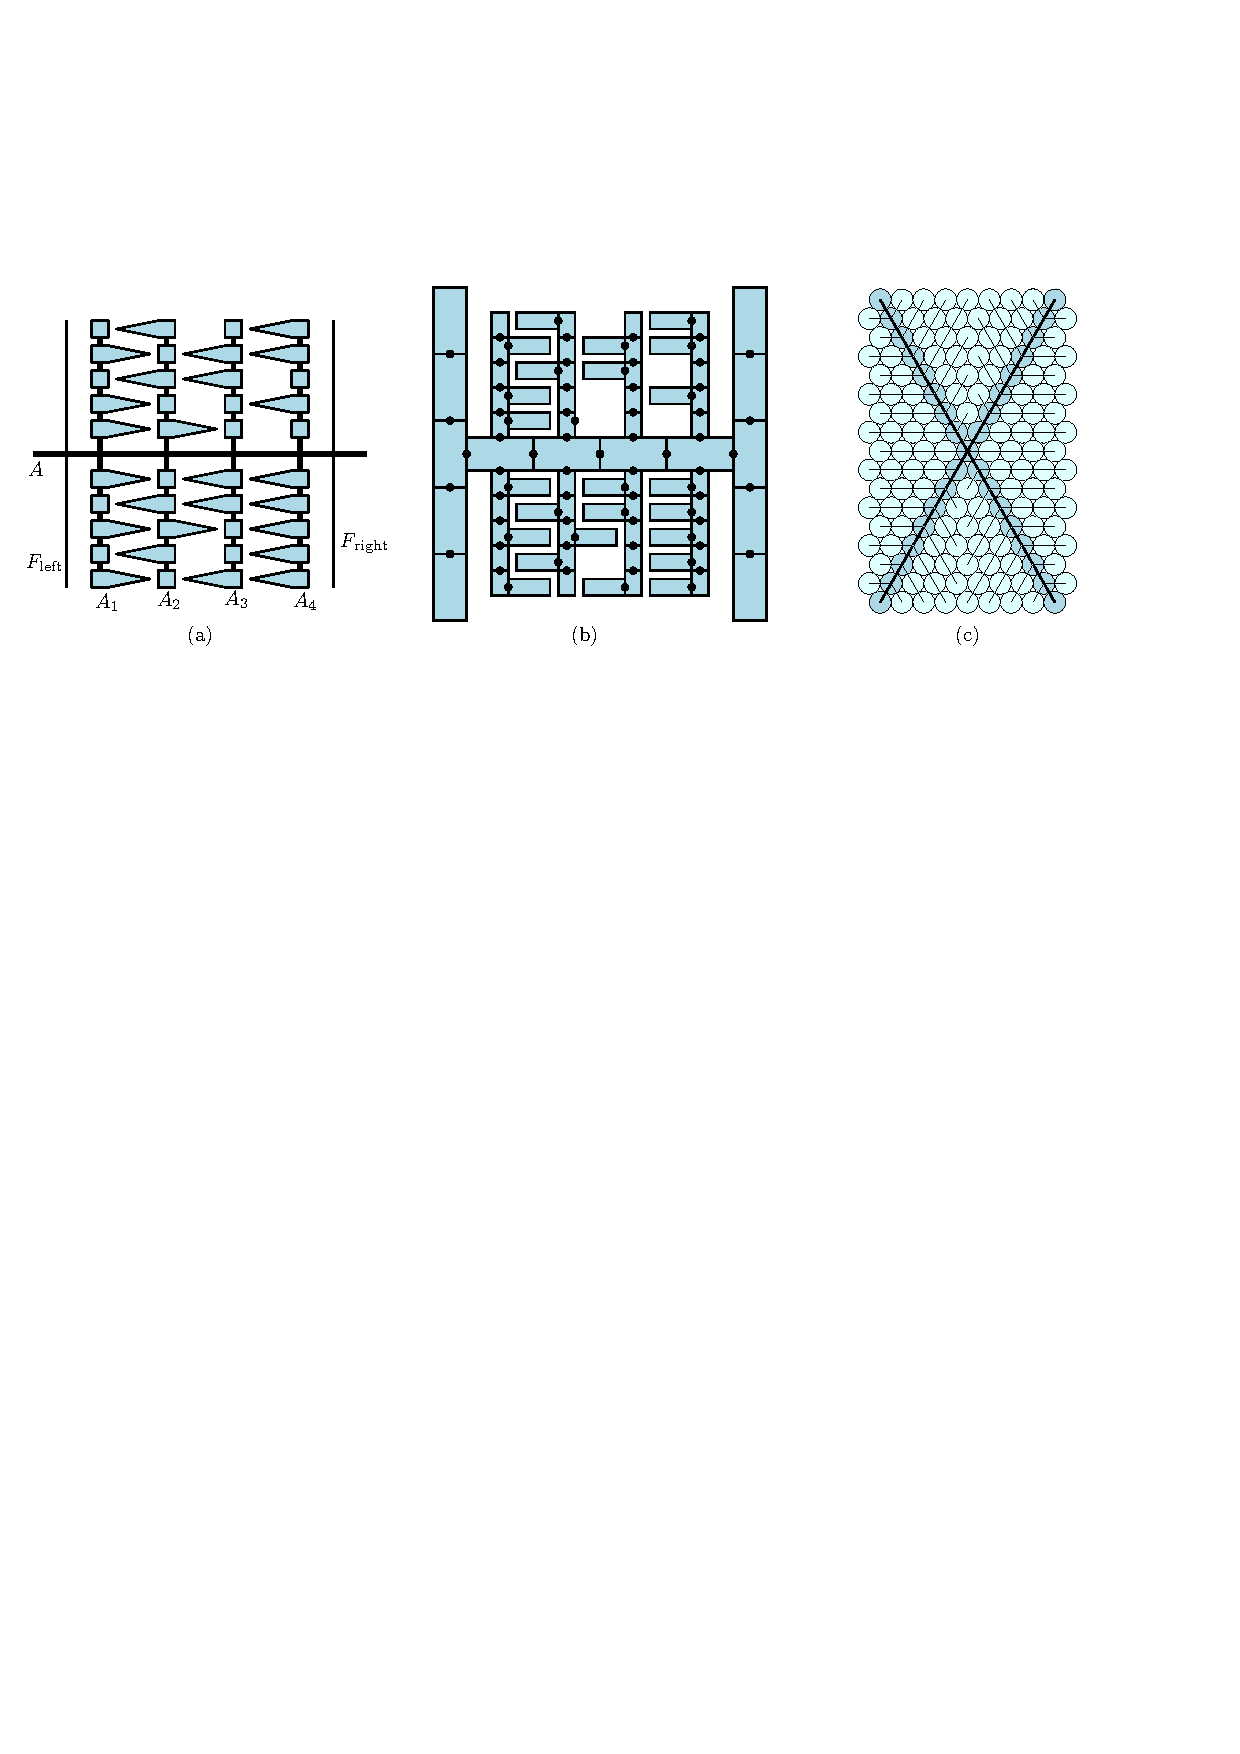
\includegraphics[width=0.95\textwidth]{fig-logic}
\caption{\small (a) A logic engine for the boolean formula for four variable and five clauses.
(b) An equivalent polygonal linkage.
(c) A disk arrangement with a cycle-free contact graph approximates a rectangle.}
  \label{fig:logic}
\end{figure}

\begin{theorem}\label{thm:hinge1}
It is NP-complete to decide whether a polygonal linkage whose hinge graph is a \emph{tree} can be realized.
\end{theorem}
\begin{proof}
We reduce NAE3SAT to the realizability of a polygonal linkage with a tree hinge graph. For a logic engine associated to an instance of NAE3SAT, we construct a polygonal linkage of polynomial size, built of rectangles. Refer to Fig.~\ref{fig:logic}(b). Every axis and each frame is replaced by a chain of rectangles hinged together at points on the axes. Each flag is replaced by a rectangle hinged to a rectangle of the corresponding axes. Every hinge lies on the edges of two rectangles, and so it allows a reflection about the line orthogonal to the edge and passing through the hinge. It is not difficult to see that the logic engine has a configuration with pairwise disjoint flags if and only if the polygonal linkage is realizable.
\end{proof}

Modeling the logic engine with polygonal linkages requires reflected copies of the rectangles. For an oriented realization, we use a different technique in Section~\ref{sec:hinge}. The above proof can be adapted to the realization of contact trees of disks by approximating rectangles with disk arrangements. In this context,
we say that a weighted graph $G$ is a \emph{$\varepsilon$-approximation} of a polygon $P$ if
$G$ is realizable as a contact graph of disks of given radii, and in every such realization,
the Hausdorff distance between the union of disks and a congruent copy of $P$ is at most $\varepsilon$.
A weighted graph $G$ is a \emph{stable} $\varepsilon$-approximation if, in addition,
for every two such realizations of $G$, the distance between the centers of the corresponding
disks is at most $\varepsilon$ after a suitable rigid transformation.

\begin{lemma}\label{lem:approx1}
For every $k\in \mathbb{N}$, there is a tree $T$ with vertex weights $1$ and $1-k^{-3}$ such that
it is a stable $O(k^{-1})$-approximation of a rectangle with aspect ratio $\sqrt{3}$.
\end{lemma}
\begin{proof}
Consider a $k \times (\sqrt{3}k)$ rectangle section of a triangular lattice, and place disks of radius $\frac{1}{2}$ at each grid point as in Fig.~\ref{fig:logic}(c). The contact graph of these disks contains cycles. Consider the spanning tree $T$ of the contact graph indicated in Fig.~\ref{fig:logic}(c). The tree $T$ decomposes into paths of collinear edges: $T$ contains two paths along the two main diagonals, each containing $2k-1$ vertices; all other paths have an endpoint on a main diagonal. We now modify the disk arrangement to ensure that its contact graph is $T$. The disks along the main diagonal do not change. We reduce the radii of all other disks by a factor of $1-k^{-3}$ (as a result, they lose contact with other disks), and then  successively translate them parallel
i the direction of the shortest path in $T$ to the main diagonal until the contact with the adjacent disk is reestablished. The Hausdorff distance between the union of these disks and the initial $k \times (\sqrt{3}k)$
rectangle is clearly less than 1.

However, the contact tree $T$ with these radii no longer has a unique realization (small perturbations are possible). To show stability, we argue by induction on the hop distance from the central disk. There are $O(i)$ disks at $i$ hops from the central disk, most one which have radius $(1-k^{-3})\frac{1}{2}$. Since all radii are $\frac{1}{2}$ or $(1-k^{-3})\frac{1}{2}$, the six neighbors of the central disk can differ from the regular hexagon by at most $O(k^{-3})$.  Similarly, the disks at $i$ hops from the center be off from the triangular grid pattern by
$O(i^2 k^{-3})$, for $i=1,2,\ldots , k$.
\end{proof}

\begin{theorem}\label{thm:disk1}
It is NP-complete to decide whether a given tree with positive vertex weights
is the contact graph of a disk arrangements with specified radii.
\end{theorem}
\begin{proof}
We extend the proof of Theorem~\ref{thm:hinge1}, and reduce NAE3SAT to the recognition of weighted contact graphs of disks in the plane. By Lemma~\ref{lem:approx1}, a rectangle of aspect ratio $\sqrt{3}$ can be approximated by an arrangement of disks with a tree contact graph; and a hinge can be modeled by a single disk.

Given an instance of NAE3SAT, we construct a polygonal linkage as in the proof of Theorem~\ref{thm:hinge1}, using rectangles of aspect ratio $\sqrt{3}$. The shorter sides of the rectangles along the axes and the frame have length $3k$, and $2k$ for the flags, where $k$ is the total number of variables and clauses in the boolean formula. Finally, we construct a weighted tree: replace each rectangle with the contact tree of the approximation as described above; and replace each hinge with a new vertex adjacent to
two suitable vertices of the two trees corresponding to the rectangles. The resulting weighted tree is the contact graph of a disk arrangement with the given radii iff the polygonal linkage is realizable.
\end{proof}


\section{Oriented Realizability of Polygonal Linkages\label{sec:hinge}}

Our proof for Theorem~\ref{thm:hinge} is a reduction from {\sc Planar-3-SAT} (P3SAT): decide whether a given a Boolean formula in 3-CNF with a planar associated graph is satisfiable. The \emph{graph associated} to a Boolean formula in 3-CNF is a bipartite graph where the two vertex classes correspond to the variables and to the clauses, respectively; and there is an edge between a variable $x$ and a clause $C$ iff $x$ or $\neg x$ appears in $C$. See Fig.~\ref{fig:assoc}(left).
Knuth and Raghunathan~\cite{KR92} point out that we may assume that the associated graph has an
embedding in the integer grid such that each variable node corresponds to a horizontal segment on
the $x$-axis, the clause nodes lie above or below that line, and each edge consists of a vertical and a possible horizontal segment.

\begin{figure}[htbp]
	\centering
	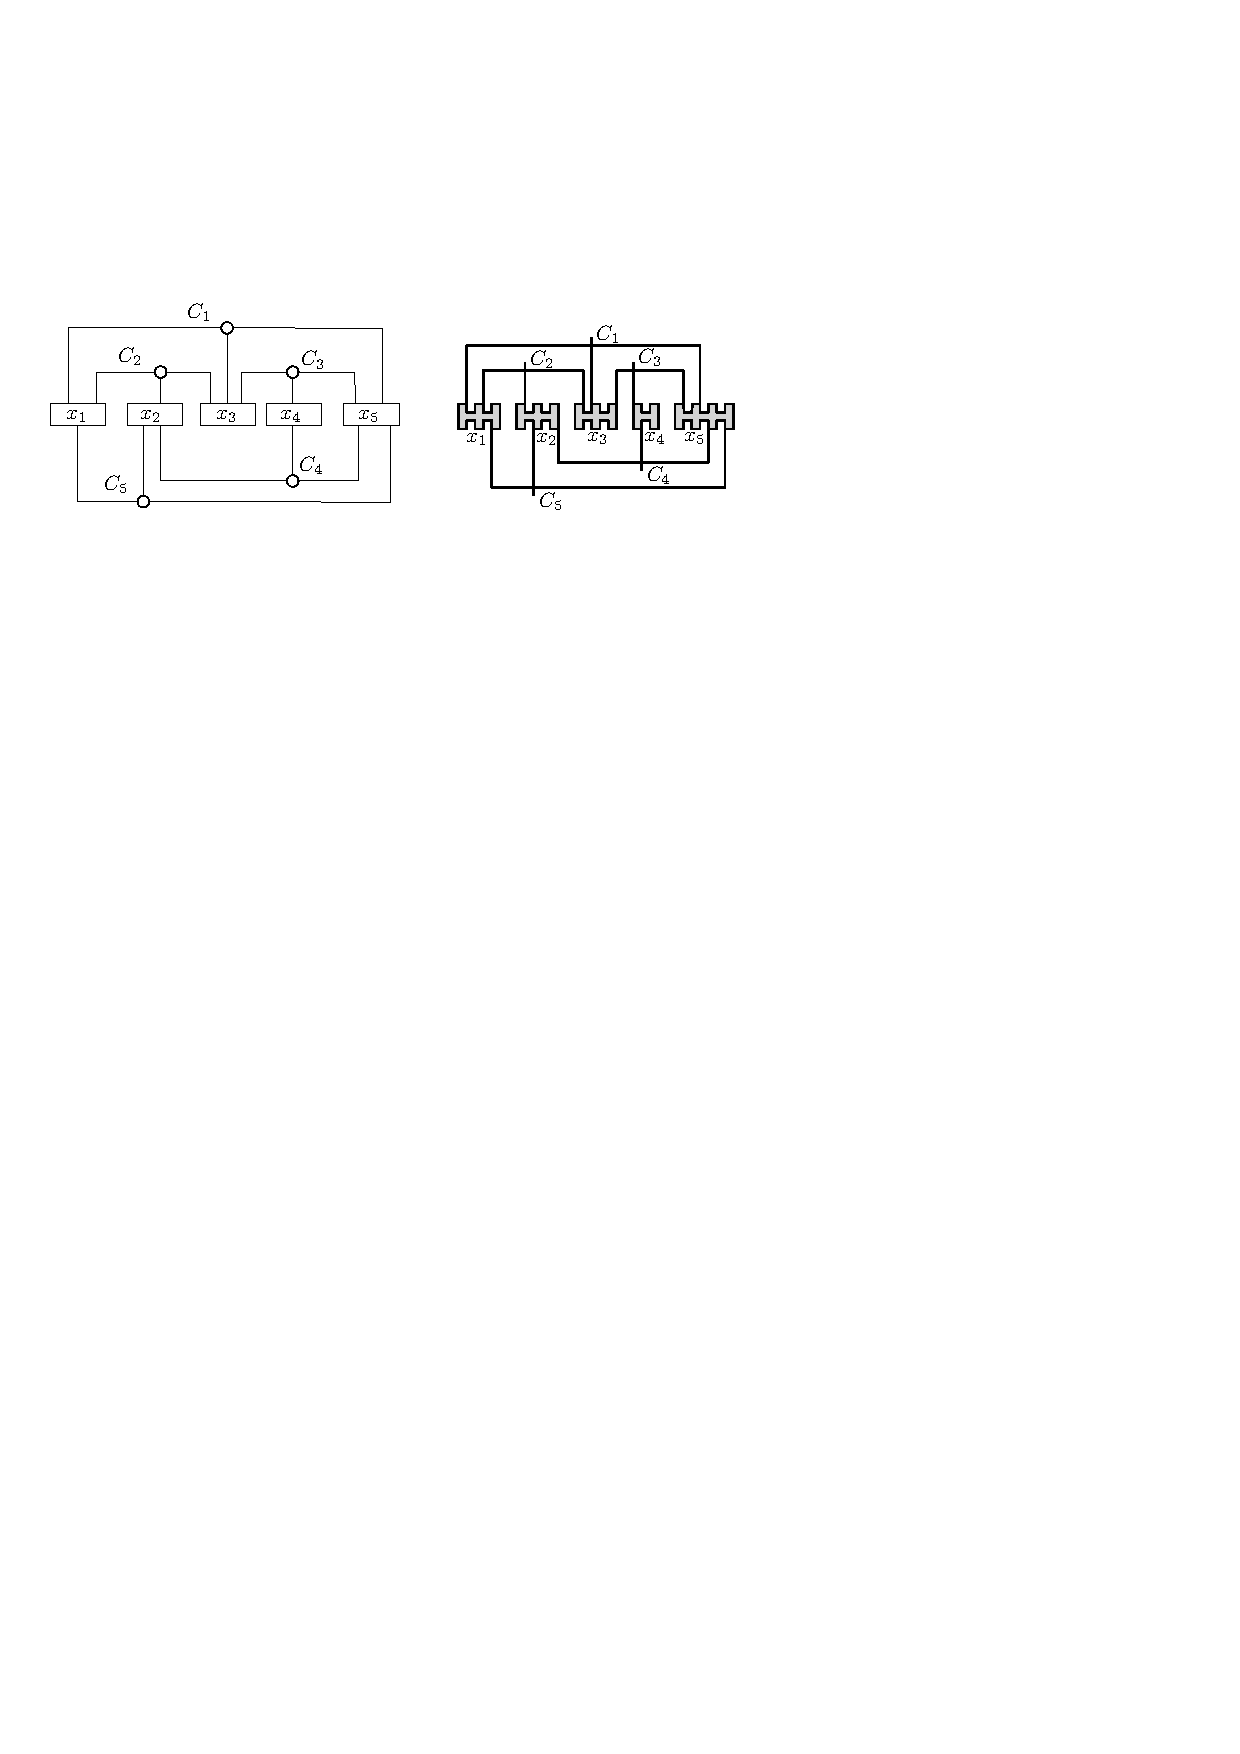
\includegraphics[width=0.7\columnwidth]{fig-assoc}
	\caption[]{Left: the associated graph $A(\Phi)$ for a Boolean formula $\Phi$.
Right: the schematic layout of the variable, clause, and transmitter gadgets in our construction.}
	\label{fig:assoc}
\end{figure}


\paragraph{The big picture.}
Given an instance $\Phi$ of P3SAT with $n$ variables and $m$ clauses, we construct a simply connected polygonal linkage $(\PP,H)$, of polynomial size in $n$ and $m$, such that $\Phi$ is satisfiable iff $(\PP,H)$ has an oriented realization. We construct a polygonal linkage  in two main steps: First, we construct an auxiliary structure where some of the polygons have fixed position in the plane (called \emph{obstacles}), while other polygons are flexible, and each flexible polygon is hinged to an obstacle. Second, we modify the auxiliary construction into a polygonal linkage by allowing the obstacles to move freely, and by adding new polygons and hinges as well as an exterior \emph{frame}.

The main idea for the auxiliary construction is the following. We start with a grid embedding of the graph $A(\Phi)$ associated to $\Phi$, and replace the vertices by variable and clause gadgets, and the edges by ransmitter gadgets (to be described below). We represent the edges of the integer grid by horizontal and vertical \emph{corridors} of uniform width. The boundaries of the corridors form squares, one square in the interior of each grid cell, which will be the obstacles polygons in our auxiliary construction. In each corridor, we insert flexible squares, with one corner hinged to
the boundary of the corridor. Each of flexible square has two possible realizations (\emph{left} and \emph{right}), see Fig.~\ref{fig:variable}(a-b). We use the spacing between the flexible squares to control how the state of one square impacts the states of adjacent squares. With suitable spacing, the state of one square may determine the state of all squares in a chain. This phenomenon helps designing variable and transmitter gadgets. Some of the squares can protrude from a corridor into an intersection (where 4 corridors meet): with proper spacing of the hinges, we can ensure that no two squares can enter an intersection, and simulate a clause by a single intersection (Fig.~\ref{fig:clause}).

\paragraph{Auxiliary Construction: flexible squares in a rigid frame.}
Let $t\in \mathbb{N}_0$ be a nonnegative integer (to be specified later). Let $\Phi$ be a Boolean formula in 3CNF with variables $x_1,\ldots , x_n$ and clauses $C_1,\ldots ,C_m$, and let $A(\Phi)$ be the associated planar graph. Consider an embedding of $A(\Phi)$ in the integer grid (Fig.~\ref{fig:assoc}) such that each variable node corresponds to an axis-aligned rectangle along the $x$-axis, the clause nodes lie above or below the $x$-axis, and each edge consists of a vertical and a possible horizontal segment~\cite{KR92}. Refine the grid, by adding extra lines $x=i+\frac{1}{2}$ and $y=j+\frac{1}{2}$ for $i,j\in \mathbb{N}$. The grid embedding of $A(\Phi)$ lies in an $N\times N$ section of the integer grid, where $N$ is a polynomial of $n$ and $m$. Scale up the refined grid by a factor of $10+3t$.
Represent the edges of the grid by horizontal and vertical \emph{corridors} of width 1. The holes between the corridors are $(4+3t/2)\times (4+3t/2)$ squares, which are considered fixed obstacles in our auxiliary construction. We need to describe variable, clause, and transmitter gadgets.

The basic building block of both variable and transmitter gadgets consists of $3+t$ unit squares hinged to the bottom or left wall of a corridor such that the hinges divide the wall into $4+t$ intervals of length $(\alpha, 2-\alpha, \frac{3}{2},\frac{3}{2},\ldots, \frac{3}{2}, 2-\beta, \beta)$ for appropriate $\alpha,\beta\in [0,1]$, as shown in Fig.~\ref{fig:variable}(a-b) for $t=0$. We call this  an $(\alpha,\beta)$-corridor. Since the height of the corridor is 1, each square has two possible orientations: it lies either \emph{left} or \emph{right} of the hinge in a horizontal corridor (above or below in a vertical corridor). For simplicity, we use the same notation (R for above, L for below) in vertical corridors. Hence, the \emph{state} of each flexible square in a realization is either L or R. The following observation describes the key mechanism of our construction.

\begin{observation}\label{obs:ab}
\begin{itemize}%\itemsep -2pt
\item[]
\item If the leftmost square is in state R, then all three squares are in state R, and the rightmost square occupies $1-\beta$ portion of the intersection on the right of the corridor.
\item Similarly, if the rightmost square is in state L, then all three squares are in state L, and the leftmost square occupies $1-\alpha$ portion of the intersection on the left  of the corridor.
\item If a square from one corridor occupies part of an intersection, then no square from the two  orthogonal corridors can occupy any part of that intersection.
\item If $\alpha,\beta>\frac{1}{2}$, then at most one square can enter an intersection.
\end{itemize}
\end{observation}


The {\bf variable gadget} for variable $x_i$ consists of $(\frac{1}{2},\frac{1}{2})$-corridors in a ziz-zag cycle along as indicated in Fig.~\ref{fig:variable}(c). The number of upper-left (resp., upper-right, etc.) corners of the zig-zag cycle is the degree of the variable node $x_i$ in $A(\Phi)$.
By Observation~\ref{obs:ab}, the state of any flexible square in the variable gadget determines the state of all other flexible squares. If $x_i=T$, then the upper-left corner of the zig-zag is occupied by a square from a vertical $(\frac{1}{2},\frac{1}{2})$-corridor; if $x_i=F$, it is occupied by a square of a vertical $(\frac{1}{2},\frac{1}{2})$-corridor.

\begin{figure}[htbp]
	\centering
	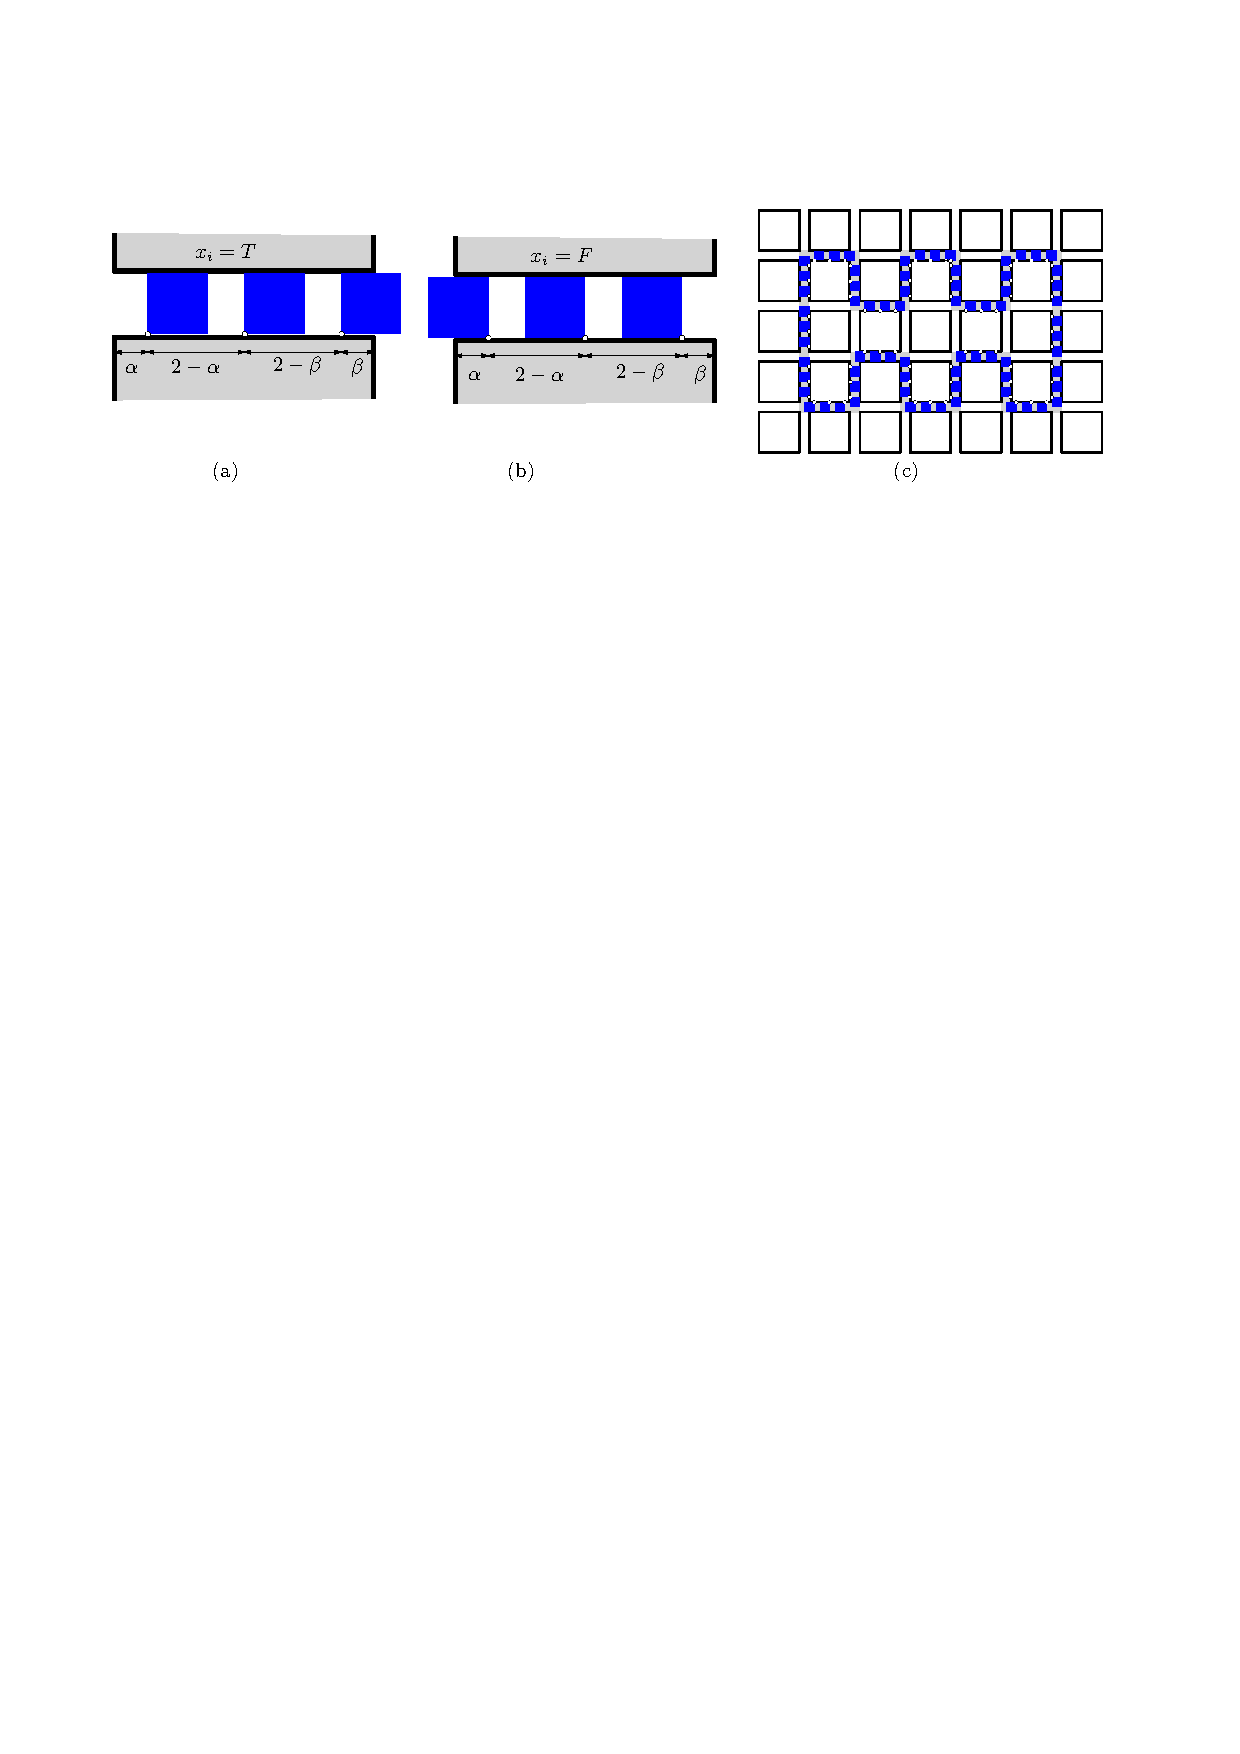
\includegraphics[width=0.95\columnwidth]{fig-variable}
	\caption{(a) Three squares in a corridor when $x_i=${\sc True}.
(b)  Three squares in a corridor when $x_i=${\sc False}.
(c) A variable gadget when $x_i=${\sc True}. }
	\label{fig:variable}
\end{figure}

A {\bf transmitter gadget} is constructed for each edge $(x_i,C_j)$ of the graph $A(\Phi)$.
It connects a corner of the variable gadget $x_i$ with the intersection representing the clause gadget $C_j$. it consists of a chain of vertical corridors and a chain of horizontal corridors. If literal $x_i$ (resp., $\overline{x}_i$) appears in $C_j$, then it is docks to an upper-left or lower-right (resp., upper-right or lower-left) corner of the variable gadget. A $(\frac{1}{2},\frac{1}{4})$-corridor docks to the variable gadget (with $\alpha=\frac{1}{2}$ adjacent to the variable gadget), an $(\frac{1}{4},1)$-corridor docks to the clause gadget, and $(\frac{1}{4},\frac{1}{4})$-corridors are used in between. Observation~\ref{obs:ab} now implies the following (see Fig~\ref{fig:clause}): (1) If $x_i$ is a {\sc False} literal in $C_i$, then the last square of the transmitter gadget is facing towards the clause gadget. (2) If $x_i$ is a {\sc True} literal in $C_i$, then transmitter gadget has a realization in which the last square faces away from the clause gadget, leaving a gap at the end of the last corridor.

\begin{figure}[htbp]
	\centering
	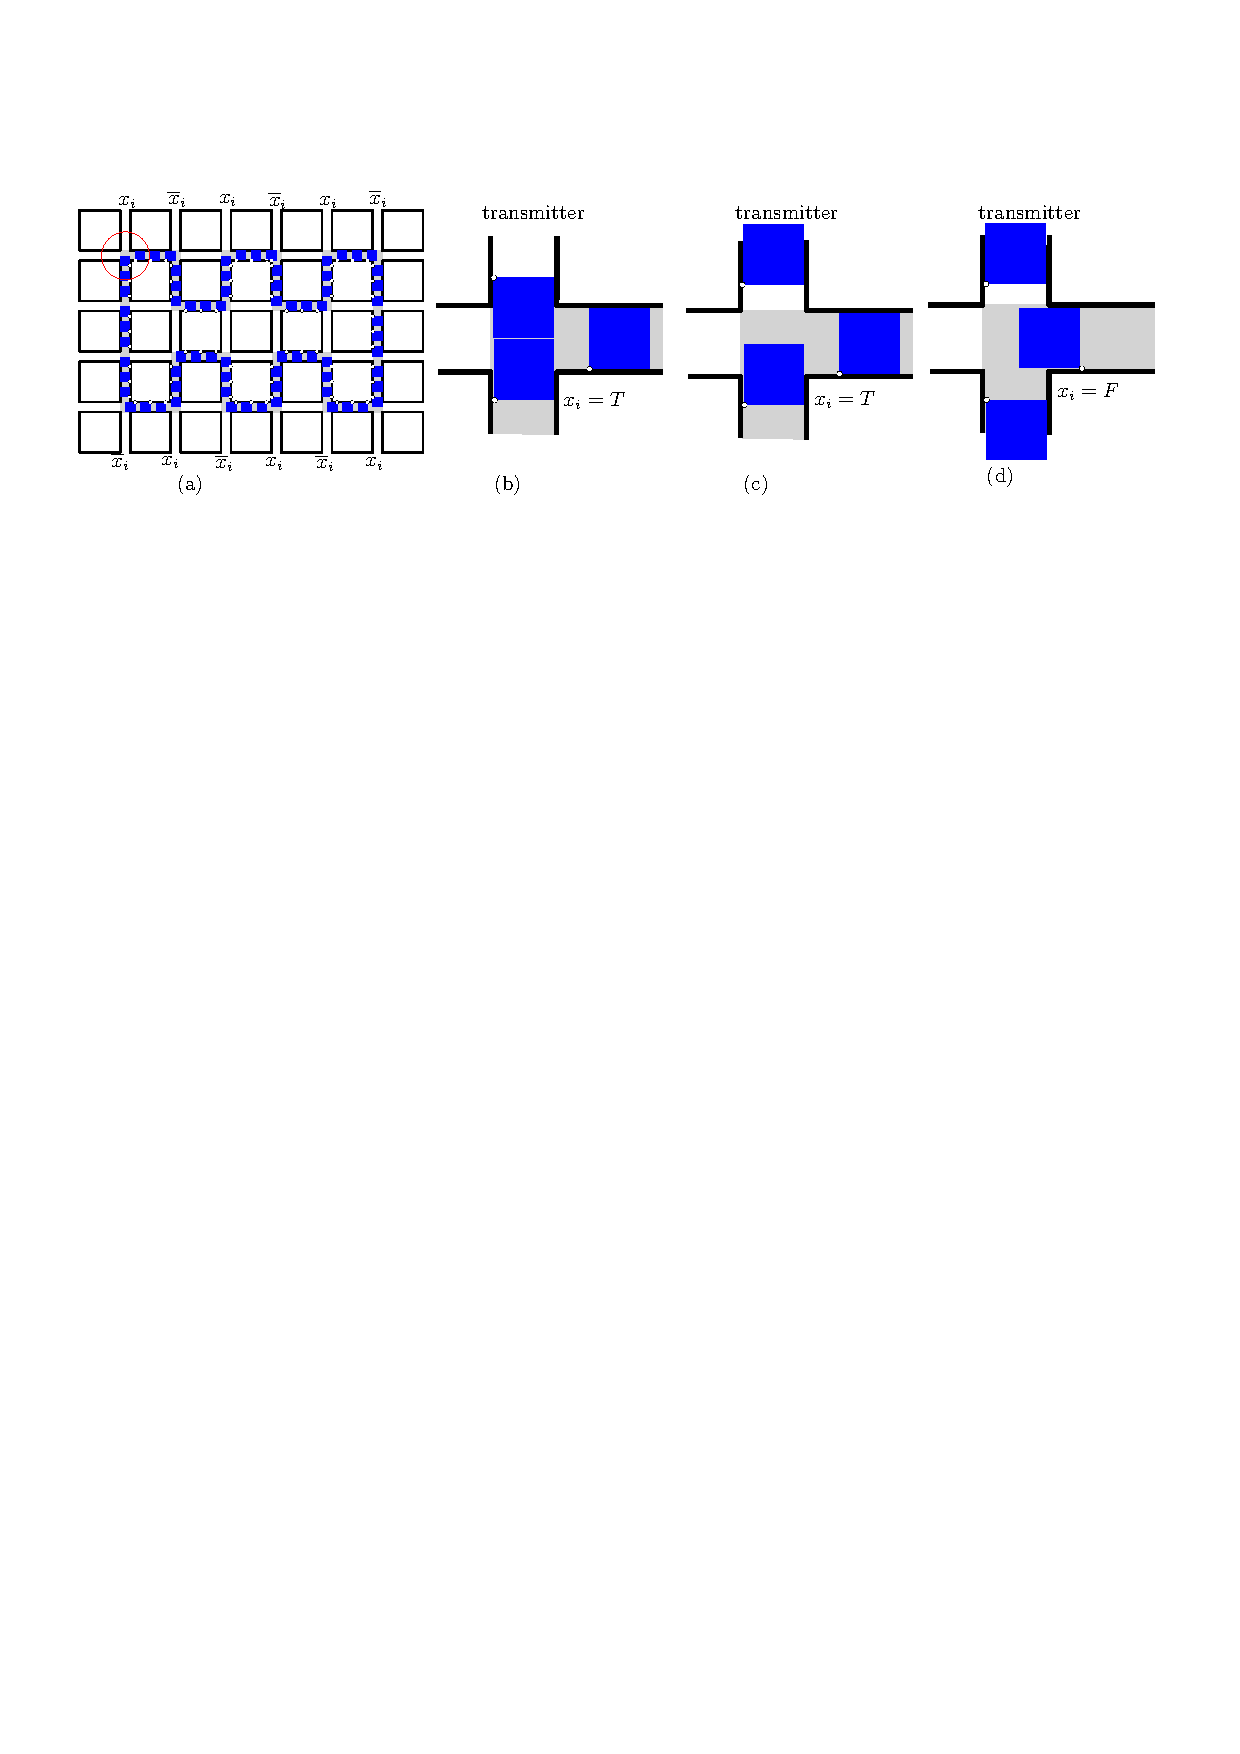
\includegraphics[width=0.95\columnwidth]{fig-transmitter}
	\caption{(a) An upper-left corner of the variable gadget $x_i$.
(b) When $x_i=T$, the first square of the transmitter may enter into an intersection of the variable gadget.
(c) When $x_i=T$, the transmitter gadget has several possible realizations.
(d) When $x_i=F$, the first square of the transmitter cannot enter into an intersection of the variable gadget.}
	\label{fig:transmitter}
\end{figure}

The {\bf clause gadget} lies at an intersection adjacent to three transmitter gadgets. The fourth corridor is a $(0,0)$-corridor, and a skinny triangle of diameter 2 is hinged to the side of the
square adjacent to the intersection, as shown in Fig.~\ref{fig:clause}. The triangle does not fit into the intersection (of diameter $\sqrt{2}$): In any realization, it must enter into a corridor of one of the three transmitter gadgets. If all three literals are {\sc False}, then this
is impossible, and no realization exists. Otherwise the triangle fits
into the empty space at the end of one of the there transmitter gadgets.

\begin{figure}[htbp]
	\centering
	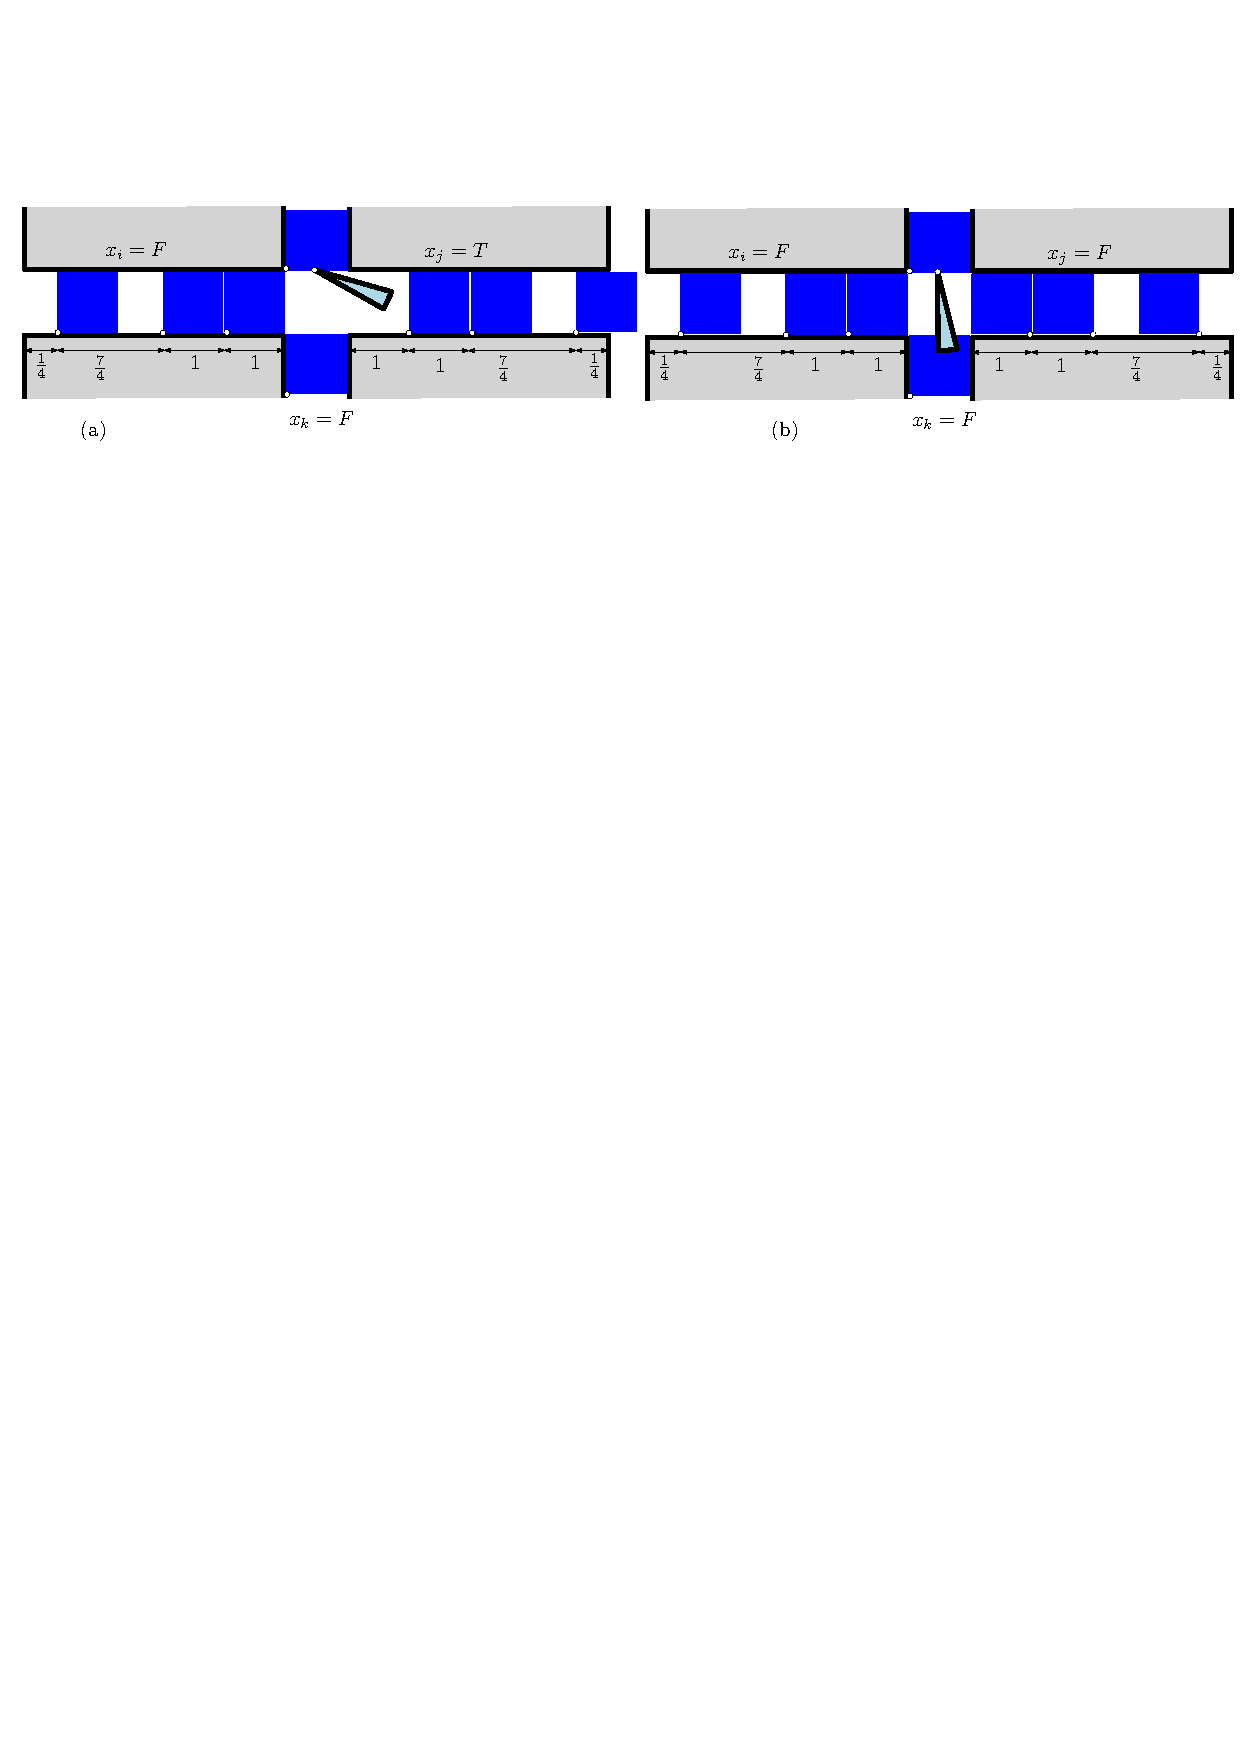
\includegraphics[width=0.95\columnwidth]{fig-clause}
	\caption{(a) A clause gadget for $C=(x_i\lor x_j\lor x_k)$ is
realizable when at least one of the literals is {\sc True}.
(b) The clause gadget cannot be realized when all three literals are {\sc False}.}
	\label{fig:clause}
\end{figure}

The following lemma summarizes or result about the auxiliary construction.
\begin{lemma}\label{lem:aux}
For every instance $\Phi$ of P3SAT, the above polygonal linkage with flexible and obstacle polygons
has the following properties: (1) it has polynomial size; (2) its hinge graph is a forest;
(3) it admits a realization such that the obstacle polygons remain fixed if and only if $\Phi$ is satisfiable.
\end{lemma}

\paragraph{Full Construction: a simply connected linkage.}
Let $\Phi$ be an instance of P3SAT (i.e., a Boolean formula $\phi$
in 3-CNF with $n$ variables, $m$ clauses, and a planar graph $A(\Phi)$).
We construct a simply connected polygonal linkage $(\PP,H)$ that has an oriented
realization iff $\Phi$ is satisfiable. We modify the auxiliary construction
by adding extra polygons and hinges, and allowing all polygons to move freely.

Recall that our auxiliary construction is based on a $(10+3t)N\times (10+3t)N$ section of the integer grid, where $N$ is a polynomial of $n$ and $m$, with $4\times 4$ obstacle squares and $1\times 1$ flexible squares. We use the auxiliary construction with parameter $t=N^2$ and modify it in 4 steps as follows.

\begin{enumerate}
\item Move the obstacle squares apart such that the width of each corridor increases from 1 to $1+1/(100N)$.
\item Add unit squares in the corridors that played no role in the auxiliary construction, using $(1,1)$-corridors.
\item Add a frame of 4 hinged rectangles around the obstacle squares as shown in Fig.~\ref{fig:frame}(a),
leaving no gap between the frame and the outer layer of obstacle squares.
\item Introduce a hinge at the midpoint of the bottom side of each obstacle square.
In the bottom row of obstacles, this point is hinged to the frame.
In all other obstacles, this point is hinged to a new \emph{connector}
polygon: a skinny rhombus of diameter 1 and width $1/(200N)$.
The far corner of each rhombus is hinged to the flexible unit square
at the midpoint of the opposite side of the corridor at shown
in Fig.~\ref{fig:frame}(b).
\end{enumerate}

\begin{figure}[htbp]
	\centering
	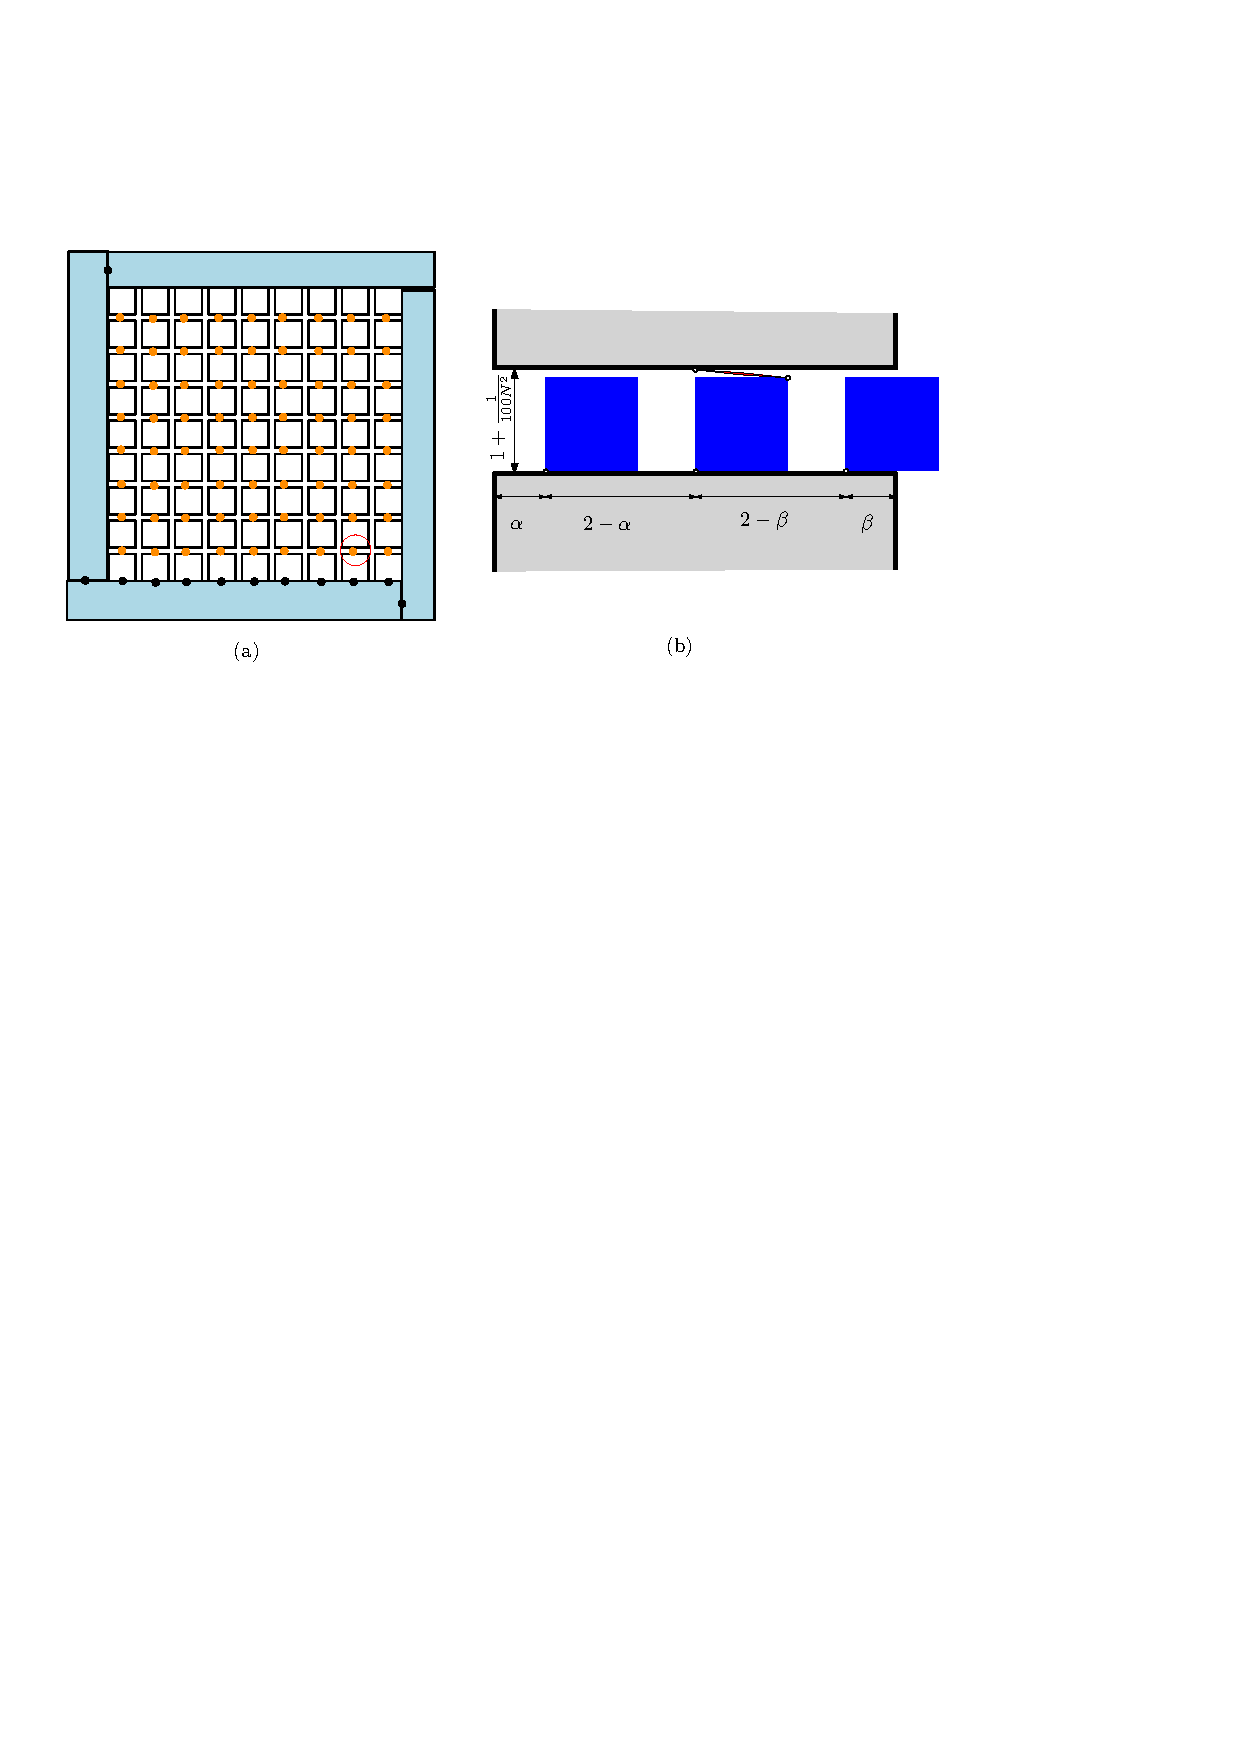
\includegraphics[width=0.95\columnwidth]{fig-frame}
	\caption{(a) A frame (built of 4 hinged rectangles) encloses an $N\times N$ grid, and
    a zig-zag path connects all obstacle squares.
    (b) A corridor is widened to $1+1/N^2$. A connection between two adjacent obstacle squares is
     established via a skinny rhombus.}
	\label{fig:frame}
\end{figure}

We obtain a simply connected polygonal linkage. We now allow the ``obstacle'' squares
to move freely, and call their original fixed position \emph{canonical}. We may assume
w.l.o.g. that the frame is at its original position. It is enough to show that the obstacle
squares are still confined to an $1/N$-neighborhood of their canonical position, then it
follows that the polygonal linkage is realizable if and only if $\Phi$ is satisfiable.

The obstacle squares in the bottom row are hinged directly to the frame, and so they are
locked in their canonical position. Consider two obstacle squares on opposite sides of a
horizontal corridor. The distance between the midpoint of the bottom and top side of the
corridor is at least 1 (due to the unit squares in the corridor) and at most 2
(due to the connector polygon). The side length of the obstacle rectangles is much larger,
$(10+3N^2)N$, so the orientations of the two adjacent obstacles differ by at most
$1/N^2$. Consequently, the orientation of \emph{any} obstacle differs from
axis-aligned by at most $1/N^2$. Due to the unit squares within a horizontal
corridor, the length of any vertical segment across the corridor is at least
$1-1/N^2$. The vertical distance between the bottom and top frames gives an
upper bound of  $2N/(100N^2)=1/(100N)$ for the sum of these vertical.
We conclude that the $y$-coordinates of the obstacles are within $1/(10N)$
of canonical. Due to the connector polygons, the $x$-coordinates of
two adjacent obstacles differ by either less than the vertical offset
or by about one unit. However, the horizontal distance between the left and right
frames prevent a shift of about one unit. So the $x$-coordinates of the obstacle
squares are also within $1/N$ of canonical.


\begin{theorem}\label{thm:hinge2}
It is NP-complete to decide whether a simply connected polygonal linkage admits an oriented realization.
\end{theorem}

\section{Oriented Realizability of Disk Arrangements\label{sec:disk}}

For the proof of Theorem~\ref{thm:disk1} for plane graph, we extend the reduction from the
previous section. It is enough to show that the construction with simply connected linkages
works with polygons that can be approximated with disk arrangements whose contact graphs are trees.
In Section~\ref{sec:logic}, we have seen that rectangles of aspect ratio $\sqrt{3}$ can be
approximated with such a disk arrangement (Fig.~\ref{fig:logic}(c)), and an $\varepsilon$-approximation requires an arrangement whose size is polynomial in $1/\varepsilon$. In the constructions in Section~\ref{sec:hinge}, we can replace the obstacle polygons and the frame polygons with rectangles of aspect ratio of about $\sqrt{3}$ (by using different lengths for horizontal and vertical corridors); and we can replace a connector polygons with a chain or disks of radius $1/(200N^2)$.

However, it was crucial in the argument that the flexible unit squares have the same width and height: this ensured that they each have exactly two possible realizations in the auxiliary construction.
We replace the unit squares with \emph{regular hexagons}. Note that if a corner of a regular hexagon of side length 1 is hinged to the boundary of a corridor of width $\sqrt{3}$, then the hexagon  has exactly two realizations. By adjusting the size of the corridors, our auxiliary construction in Section~\ref{sec:hinge} can be built with (approximate) rectangles of aspect ratio $\sqrt{3}$ and regular hexagons.

\begin{figure}[htbp]
  \centering
 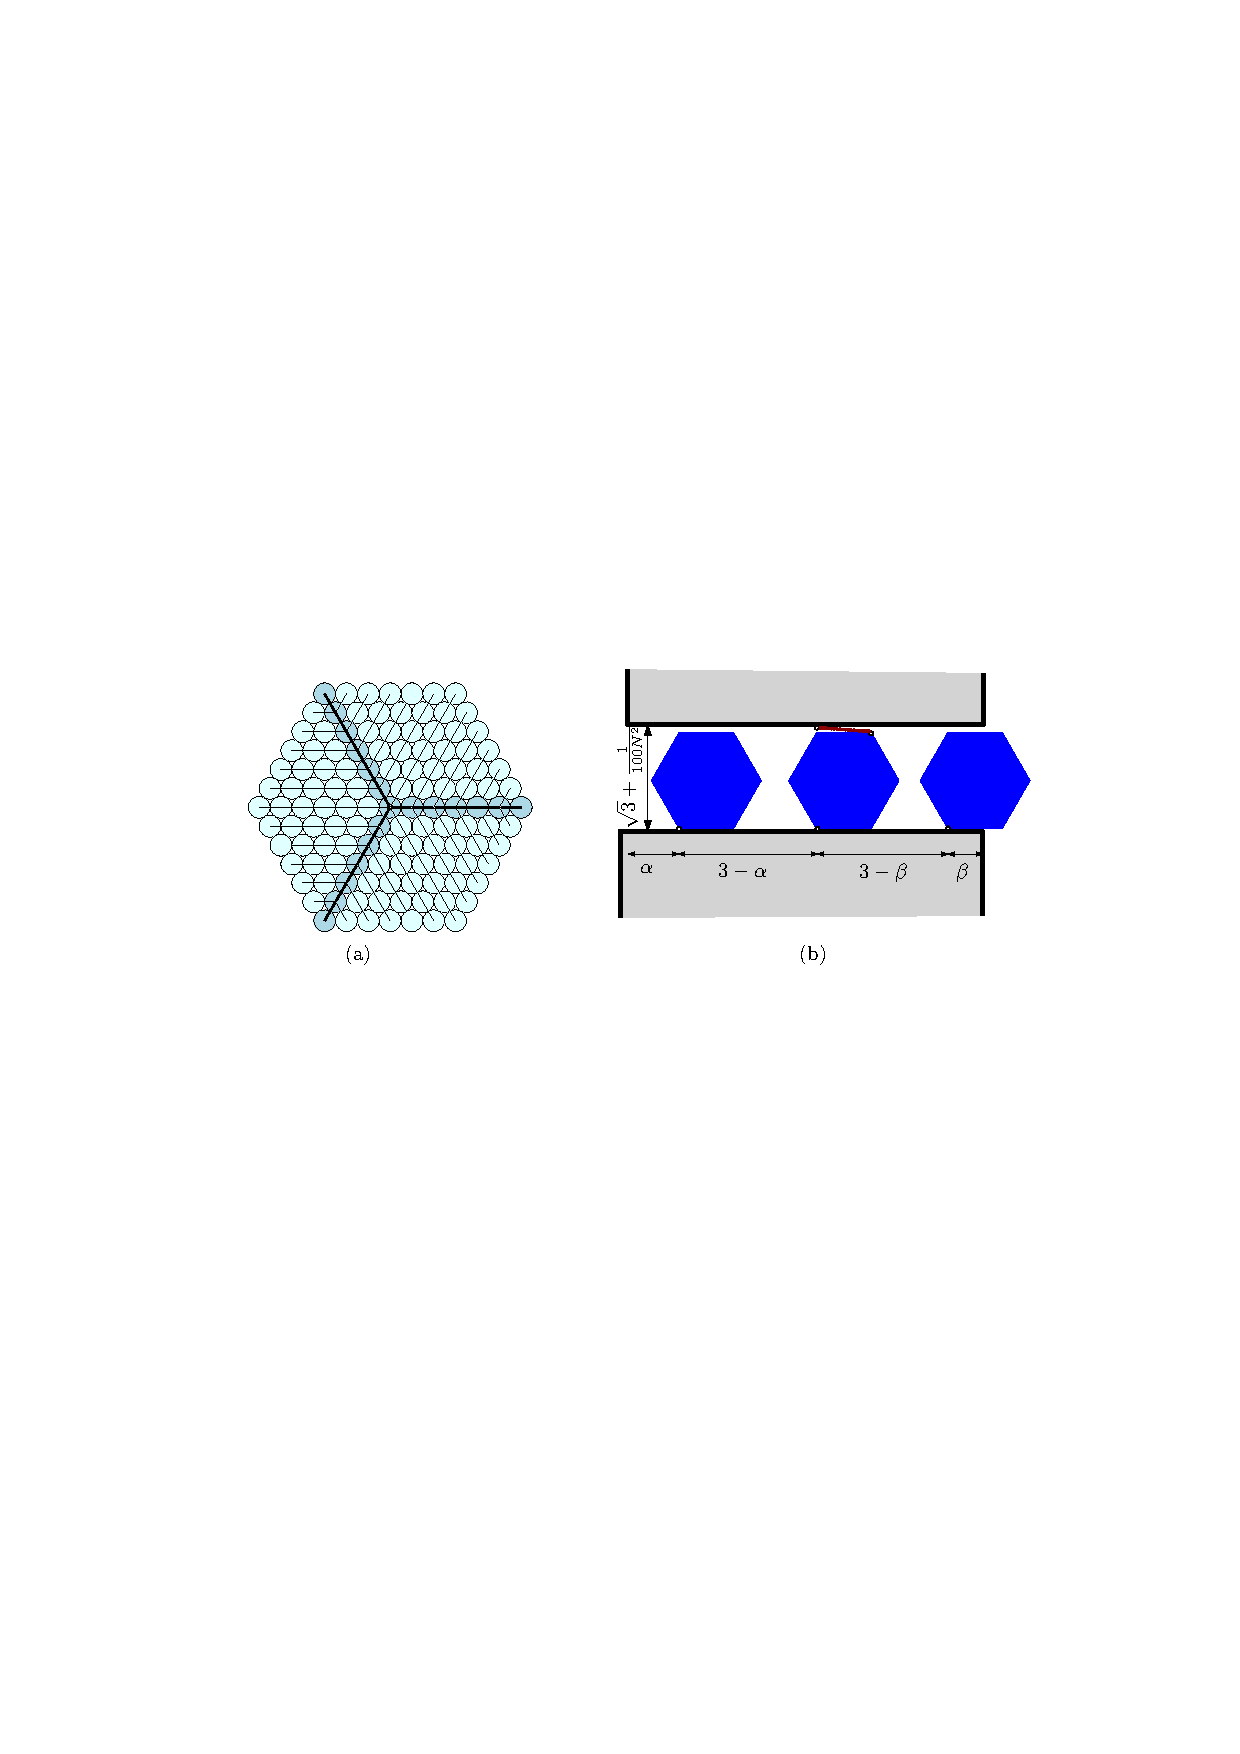
\includegraphics[width=0.8\textwidth]{fig-hexagon}
\caption{\small A disk arrangement with a cycle-free contact graph approximates a regular hexagon.}
  \label{fig:hexagon}
\end{figure}

\begin{lemma}\label{lem:approx2}
For every $k\in \mathbb{N}$, there is a tree $T$ with vertex weights $1$ and $1-k^{-2}$ such that
every disk arrangement with contract graph $T$ and given weights is an $O(1/k)$-approximation of a regular hexagon.
\end{lemma}
\begin{proof}
Consider a regular hexagon section of a triangular lattice, with side length $k$, and place disks of radius $\frac{1}{2}$ at each grid point. Consider the spanning tree $T$ of the contact graph indicated in Fig.~\ref{fig:hexagon}(b). The tree $T$ decomposes into paths of collinear edges: three \emph{backbone} paths of length $k$ that connect the center to 3 pairwise nonadjacent corners of the hexagon; all other paths have an endpoint on a backbone. We now modify the disk arrangement to ensure that its contact graph is $T$. The disks along the backbones do not change; but we reduce the radii of all other disks by a factor of $1-k^{-3}$, and translate them successively in the direction of the path to a backbone until the contact with the adjacent disk is reestablished. The Hausdorff distance between the union of these disks and the initial hexagon is clearly less than 1.
Stability can be shown by induction analogously to Lemma~\ref{lem:approx1}.
\end{proof}


\begin{theorem}\label{thm:disk2}
It is NP-complete to decide whether a given plane tree with positive vertex weights
is the contact graph of an oriented disk arrangement with specified radii.
\end{theorem}


\section{Conclusions \label{sec:con}}

We have shown that deciding whether a simply connected polygonal linkage is realizable in the plane (with or without given orientations) is NP-hard. Previously, NP-hardness was known only for linkages with high genus. A polygonal linkage is simply connected when its hinge graph (in which two polygons are adjacent if they are hinged together) is a tree. It remains an open problem whether the realizability polygonal linkages whose hinge graphs are \emph{paths}
is solvable in  polynomial time.

Our proof technique (the approximation of polygons by disk arrangements) used disks of radius close to one. It remains an open problem whether recognizing contract trees of \emph{unit} disks in the plane is NP-hard. We believe it is, but it would require an approximation of a ``dense'' unit disk packing with an arrangement of unit disks whose contact graph is a tree: this leads to challenging approximation problems in discrete geometry. We used contact trees of degree 6 for stable $\varepsilon$-approximations. It would be interesting to see whether the realizability of weighted graphs (as contact graphs of disks) remains NP-hard for trees of maximum degree 5, 4, or 3.

We have shown that four decision problems are NP-hard. We do not know whether the related optimization problems can be approximated efficiently. Specifically, partition a given polygonal linkage into the minimum number of realizable pieces; or find the largest subtree of a weighted tree that is the contact graph of disks of the corresponding radii.


\begin{thebibliography}{99}
\itemsep -1pt

\bibitem{AKR+04}
H. Alt, C. Knauer, G. Rote, and S. Whitesides,
On the complexity of the linkage reconfiguration problem,
in \emph{Towards a Theory of Geometric Graphs},
vol.~342 of Contemporary Mathematics, AMS, 2004, pp.~1--14.

\bibitem{BCD+09}
B.~Ballinger, D.~Charlton, E.~D. Demaine, M.~L. Demaine,
J.~Iacono, C.-H.~Liu, S.-H.~Poon,
Minimal locked trees,
in \emph{Proc. 11th WADS}, LNCS~5664, Springer, 2009, pp.~61--73.

\bibitem{BC87}
S.~N. Bhatt and S.~S. Cosmadakis,
The complexity of minimizing wire lengths in VLSI layouts,
\emph{Inform. Process. Lett.} {\bf 25} (4) (1987), 263--267.

\bibitem{BK95}
H. Breu and D.~G. Kirkpatrick,
On the complexity of recognizing intersection and touching graphs of discs,
in \emph{Proc. Sympos. Graph Drawing}, LNCS~1027, Springer,  1995, pp.~88--98.

\bibitem{BK98}
H.~Breu and D.~G. Kirkpatrick,
Unit disk graph recognition is NP-hard,
\emph{Comput. Geom.} {\bf 9} (1998) 3--24.

\bibitem{CDR07}
S.~Cabello, E.~D.~Demaine, and G.~Rote,
Planar embeddings of graphs with specified edge lengths,
\emph{J.~Graph Alg. Appl.} {\bf 11} (1) (2007), 259--276.

\bibitem{CdG+07}
J.-S. Cheong, A.~F.~van der Stappen, K. Goldberg, M. H.~Overmars, and E.~Rimon,
Immobilizing hinged polygons,
\emph{Int. J. Comput. Geom. Appl.} {\bf 17} (1) (2007), 45--70.

\bibitem{CD-ch9}
R.~Connelly and E.~D. Demaine,
Geometry and topology of polygonal linkages, ch.~9 in
in \emph{Handbook of Discrete and Computational Geometry}, 2nd ed., 2004, CRC, pp.~197--218.

\bibitem{CDR03}
R.~Connelly, E.~D.~Demaine, and G.~Rote,
Straightening polygonal arcs and convexifying polygonal cycles.
\emph{Discrete Comput. Geom.} {\bf 30} (2) (2003), 205–-239.

\bibitem{CDD+10}
R.~Connelly, E.~D.~Demaine, M.~L.~Demaine, S.~P.~Fekete, S.~Langerman,
J.~S.~B.~Mitchell, A.~Rib\'o, G.~Rote,
Locked and unlocked chains of planar shapes,
\emph{Discrete Comput. Geom.} {\bf 44} %(2)
(2010), 439--462.

\bibitem{SFM+11}
V.~G.~P. De~S\'a, G.~D. Da~Fonseca, R.~C.~S. Machado, and C.~M.~H. De Figueiredo,
Complexity dichotomy on partial grid recognition,
\emph{Theor. Comp. Sci.} {\bf 412} (22) (2011), 2370--2379.

\bibitem{BV96}
G.~Di~Battista and L.~Vismara, Angles of planar triangular graphs,
\emph{SIAM J. Discrete Math.} {\bf 9} (3) (1996), 349-–359.

\bibitem{BET+99}
G.~Di Battista, P. Eades, R. Tamassia, and I.~G. Tollis,
\emph{Graph Drawing: Algorithms for the Visualization of Graphs},
Prentice Hall, 1999.

\bibitem{EW90}
P.~Eades and N.~C.~Wormald, Fixed edge-length graph drawing is NP-hard,
\emph{Discrete Applied Mathematics} {\bf 28} (1990), 111-�134.

\bibitem{FHW97}
S.~P. Fekete, M.~E. Houle, and S.~Whitesides,
The wobbly logic engine: Proving hardness of non-rigid geometric graph representation problems,
in \emph{Proc. 5th Sympos. Graph Drawing}, LNCS~1353, Springer, 1997, pp.~272--283.

\bibitem{Gre89}
A. Gregori,
Unit-length embedding of binary trees on a square grid,
\emph{Inform. Process. Lett.} {\bf 31} (1989), 167--173.

\bibitem{Hli97}
P.~Hlin\v{e}n\'y,
Touching graphs of unit balls,
in \emph{Proc. 5th Sympos. Graph Drawing}, LNCS~1353, Springer, 1997, pp.~350--358.

\bibitem{HK01}
P.~Hlin\v{e}n\'y and J.~Kratochv\'{\i}l,
Representing graphs by disks and balls (a survey of recognition-complexity results),
\emph{Discrete Mathematics} {\bf 229} (1–3) (2001), 101--124.

\bibitem{KR92}
D.~E.~Knuth and A.~Raghunathan,
The problem of compatible representatives,
\emph{SIAM Discrete Math.} {\bf 5(3)} (1992), 422–-427.

%\bibitem{Lic82}
%D.~Lichtenstein,
%Planar formulae and their uses,
%\emph{SIAM J. Comput.} {\bf 11} (2) (1982), 329–-343.

%\bibitem{RW08}
%W.~Mulzer and G.~Rote,
%Minimum-weight triangulation is NP-hard,
%\emph{J.~ACM} {\bf 55} (2) (2008), Article 11.

\bibitem{Rei79}
J.~H.~Reif,
Complexity of the mover’s problem and generalizations,
in: \emph{Proc. 20th FoCS}, IEEE, 1979, pp.~421--427.

\bibitem{Str05}
I.~ Streinu,
Pseudo-triangulations, rigidity and motion planning,
\emph{Discrete Comput. Geom.} {\bf 34} (4) (2005), 587--635.

\end{thebibliography}

\end{document}

